\section{Exemplo 1}

\begin{quotation}
Um paciente tem sofrido de falta de ar (dispneia) e visita o médico, preocupado por ter câncer de pulmão. O médico sabe que outras doenças, como tuberculose e bronquite, são possíveis causas, além do câncer de pulmão. Ela também sabe que outras informações relevantes incluem se o paciente é fumante ou não (aumentando as chances de câncer e bronquite) e a que tipo de poluição do ar ele foi exposto. Um raio-X positivo indicaria tuberculose ou câncer de pulmão.
\end{quotation}

\subsection{Definindo os nós e valores}

Primeiro, o engenheiro do conhecimento deve identificar as variáveis ​​de interesse. Isso envolve responder à pergunta: quais são os nós a representar e quais valores eles podem assumir, ou em que estado eles podem estar? Por enquanto, consideraremos apenas os nós que assumem valores discretos. Os valores devem ser mutuamente exclusivos e exaustivos, o que significa que a variável deve assumir exatamente um desses valores por vez. Os tipos comuns de nós discretos incluem:

\begin{itemize}
\item Nós booleanos, que representam proposições, assumindo os valores binários verdadeiro (T) e falso (F). Em um domínio de diagnóstico médico, o nó Câncer representaria a proposição de que um paciente tem câncer.
\item Valores categóricos. Por exemplo, um nó de poluição pode representar a exposição de um paciente à poluição e assumir os valores {baixo, médio, alto}.
\item Valores numéricos. Por exemplo, um nó chamado Idade pode representar a idade de um paciente e ter valores possíveis de 1 a 120.
\end{itemize}

Estratégias podem ser usadas para representar a idade exata de um paciente pode ser agrupar os pacientes em grupos de diferentes idades, como {bebê, criança, adolescente, jovem, meia-idade, velho}. O truque é escolher valores que representem o domínio de forma eficiente, mas com detalhes suficientes para realizar o raciocínio necessário. A Tabela~\ref{tab:tab71} lista as variáveis usadas para análise do caso do câncer de pulmão. 

\begin{table}[t]
    \caption{Escolhas preliminares de nós e valores para o exemplo do câncer de pulmão.}
    \centering
    \begin{tabular}{|c|c|c|}
    \hline
    \textit{Variável} & \textit{Tipo}  & \textit{Valores} \\ \hline
    Poluição & Binário & \{Baixa, Alta\} \\ \hline
    Fumante & Booleano & \{Verdadeiro, Falso\}      \\ \hline
    Câncer & Booleano & \{Verdadeiro, Falso\}      \\ \hline
    Dispnéia & Booleano & \{Verdadeiro, Falso\}      \\ \hline
    Raio-X & Binário  & \{Positivo, Negativo\}  \\ \hline
    \end{tabular}
    \label{tab:tab71}
\end{table}

\subsection{Estrutura}

A estrutura ou topologia da rede deve capturar relacionamentos qualitativos entre as variáveis. Em particular, dois nós devem ser conectados diretamente se um afetar ou causar o outro, com o arco indicando a direção do efeito. Portanto, em nosso exemplo de diagnóstico médico, podemos perguntar quais fatores afetam a chance de um paciente ter câncer? Se a resposta for “Poluição e fumo”, devemos adicionar arcos de Poluição e Fumante a Câncer. Da mesma forma, ter câncer afetará a respiração do paciente e as chances de ter um resultado de raios-X positivo. Portanto, adicionamos arcos de Câncer a Dispneia e Raio-X. A estrutura resultante é mostrada na Figura~\ref{fig:fig72}. É importante notar que esta é apenas uma estrutura possível para o problema; olhamos para estruturas de rede alternativas em

\begin{figure}[t]
    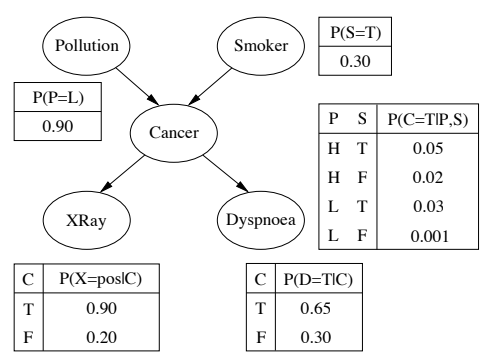
\includegraphics[width=10cm]{fig71.png}
    \centering
    \caption{Uma Rede Bayesiana para o problema do câncer do pulmão.}
    \label{fig:fig72}
\end{figure}

\subsection{Exemplo de código em R e inferência Bayesiana}

A listagem abaixo mostra o código escrito em R. O código utiliza o pacote \textsf{bnlearn} e \textsf{gRain}. A Rede Bayesiana é carregada no formato \textsf{bif} pelo arquivo \textsf{cancer.bif}. As probabilidades marginais de cada nó é representada na Figura~\ref{fig:fig81}

\begin{figure}[t]
    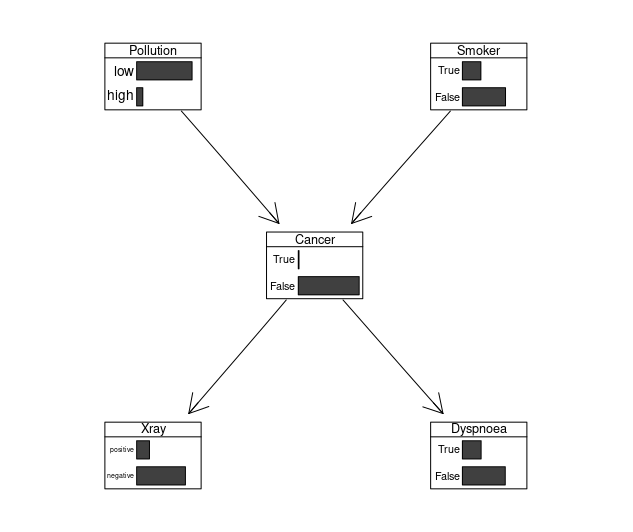
\includegraphics[width=12cm]{fig81.png}
    \centering
    \caption{Probabilidades marginais da rede Bayesiana.}
    \label{fig:fig81}
\end{figure}

São declaradas as evidências \textsf{Pollution = "high"} e \textsf{Xray = "positive"}, ou $Pr(Pollution==high) = 1$ e $Pr(Xray==positive | Cancer==true) = 1$. Consultando a probabilidade posterior antes e depois da declaração das evidências, obtém-se os resultados:

\begin{verbatim}
Cancer
   True   False 
   0.01    0.99 
\end{verbatim}

\begin{verbatim}
Cancer: Pollution = high, Xray = positive.
   True   False 
   0.12    0.88 
\end{verbatim}

Nota-se que a probabilidade de câncer de pulmão elevou de 0,01 para 0,12, dada as evidências.

\lstinputlisting[language=Octave]{code/exemplo1.r}